\documentclass{article}
\usepackage[dvipsnames]{xcolor}
\usepackage[paperwidth=20cm, paperheight=3.5cm, margin = 0cm, top=0.5cm]{geometry}

\usepackage{pgf}
\usepackage{tikz}
\usetikzlibrary{arrows,automata}
\usetikzlibrary{positioning}

\tikzstyle{source}  = [draw,circle,fill=black,thick,inner sep=0mm,minimum size=2mm]
\tikzstyle{box}  = [draw,rectangle,thick,inner sep=2mm,minimum width=8mm, minimum height=8mm]

\begin{document}
\begin{center}
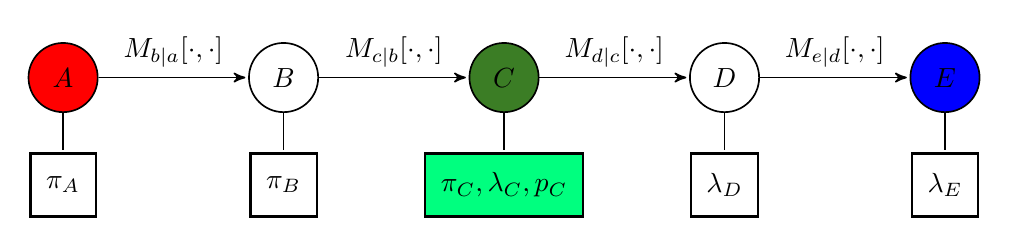
\begin{tikzpicture}[->,>=stealth',shorten >=1pt,auto,node distance=2.8cm,semithick]
                    
\node[state, fill=red] (X1)               {$A$}; 
\node[state] (X2) [right of=X1] {$B$};                   
\node[state, fill=OliveGreen] (X3) [right of=X2] {$C$};                   
\node[state] (X4) [right of=X3] {$D$};                   
\node[state, fill=blue] (X5) [right of=X4,] {$E$}; 

\node[box][below=0.5cm of X1](P1){$\pi_A$};                  
\node[box][below=0.5cm of X2](P2){$\pi_B$};
\node[box, fill=SpringGreen][below=0.5cm of X3](P3){$\pi_C,\lambda_C,p_C$};
\node[box][below=0.5cm of X4](P4){$\lambda_D$};                  
\node[box][below=0.5cm of X5](P5){$\lambda_E$};                  

\path
	(X1) edge node {$M_{b|a}[\cdot,\cdot]$} (X2)
	(X2) edge node {$M_{c|b}[\cdot,\cdot]$} (X3)
	(X3) edge node {$M_{d|c}[\cdot,\cdot]$} (X4)
	(X4) edge node {$M_{e|d}[\cdot,\cdot]$} (X5);

\path
	(X1) edge[-] (P1)
	(X2) edge[-] (P2)
	(X3) edge[-] (P3)
	(X4) edge[-] (P4)
	(X5) edge[-] (P5);

\end{tikzpicture}
\end{center}

\end{document}
